% questions.tex —— 1977 年·吉林卷 · 题目内容片段（无答案）
% 由 tools/generate_projects.py 依来源总账自 1977/1977_数学真题_吉林_试题.md 生成，勿手改（改源 MD 后重跑）


\gkpart{吉林1977年高考数学试题解}

\begin{gktip}
\textbf{来源说明}：本题面依据固定源 PDF《吉林1977年高考数学试题解》第 1—5 页（书籍页码 20—24）逐题转录。固定源是题面与解答连排的「试题解」材料，而不是无答案试卷；配套答案与解析对照源解答独立复算，非官方标准答案。原卷无文理分科与分值说明，科类栏记为不分文理。正式题按源卷大题「一、」至「六、」转录为本库第 1—6 题；第一大题含 3 个小题、第二大题含 3 个小问、第四大题含 4 个小题，源卷小题印作「1．、2．……」，本库按小问规范重排为（1）（2）……；末尾「参考题」按源卷「一、二、三」转录为参考题 1—3，不计入正式题量。源卷排印用字「园」（圆）照录；三角函数记号 Sin、Cos、tg 的大小写照录源卷，解析按现代记号 sin、cos、tan 推导。
\end{gktip}

\par\medskip

\Needspace{0.4\textheight}
\begin{question}
\gkti{1}

（1） 什么是因式分解？把 $18a^3-48a^2b+32ab^2$ 分解因式。

\Needspace{5\baselineskip}
（2） 什么是方程？什么是方程的解？解方程：

\nopagebreak[4]
\[
\frac{2}{x-2}+x=\frac{x}{x-2}.
\]

（3） 在 $\triangle ABC$ 中，$\angle C$ 是直角，$CD$ 是 $AB$ 上的高，已知 $AB=9$，$AC=6$，求 $CD$。

\begin{gktip}
原源 PDF 第 2 页附有直角三角形与斜边上的高 $CD$ 的示意图；LaTeX 版按源图重绘。
\end{gktip}
\nopagebreak[4]
\begin{center}% 1977 年吉林卷第 1 题（3）：直角三角形 ABC，∠C 为直角（带直角标记），
% CD 为斜边 AB 上的高，D 在 AB 上（按源卷第 2 页布局：B 在上、C 左下、A 右下）
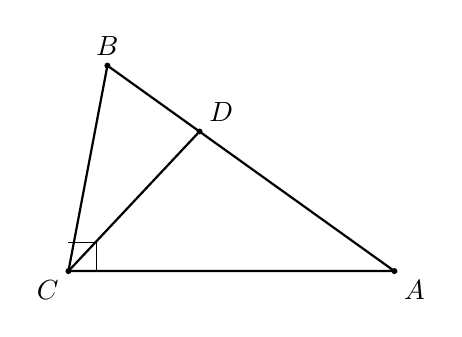
\begin{tikzpicture}[scale=0.9]
  \coordinate (C) at (0,0);
  \coordinate (A) at (4.6,0);
  \coordinate (B) at (0.55,2.9);
  \coordinate (D) at (1.85,1.97);
  \draw[thick] (A)--(B)--(C)--cycle;
  \draw[thick] (C)--(D);
  \draw (0.4,0) -- (0.4,0.4) -- (0,0.4);
  \fill (A) circle (1.2pt) node[below right] {$A$};
  \fill (B) circle (1.2pt) node[above] {$B$};
  \fill (C) circle (1.2pt) node[below left] {$C$};
  \fill (D) circle (1.2pt) node[above right] {$D$};
\end{tikzpicture}
\end{center}
\nopagebreak[4]
\end{question}
\begin{question}
\gkti{2}$k$ 是什么值时，方程 $x^2+4x+k=0$ 有

（1） 两个不相等的实根？

（2） 相等的实根？

（3） 没有实根？

\Needspace{0.4\textheight}
\end{question}
\begin{question}
\gkti{3}什么是平面上的轨迹？

某港口外海面上，有一个暗礁区，为进港船只的安全，建有 $A\text{、}B$ 两灯塔，把暗礁区所张的危险的角 $\angle AMB$ 的大小通知船上。试用轨迹涵义证明：只要进港船只 $S$ 的视角 $\angle ASB<\angle AMB$ 时，船只就可安全进港。

\begin{gktip}
原源 PDF 第 2 页附有灯塔 $A\text{、}B$、圆弧上的点 $M$ 与船只 $S$ 的示意图；LaTeX 版按源图重绘。
\end{gktip}
\nopagebreak[4]
\begin{center}% 1977 年吉林卷第 3 题：港口暗礁轨迹示意——圆内弦 AB、圆周角顶点 M（在圆上）
% 与圆外船只 S，S、M、B 共线，另画 SA 与 AM（按源卷第 2 页布局：S 在上、AB 在下）
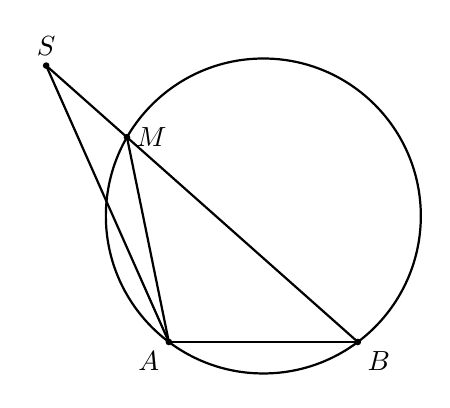
\begin{tikzpicture}[scale=1.0]
  \draw[thick] (0,0) circle (2);
  \coordinate (A) at (-1.2,-1.6);
  \coordinate (B) at (1.2,-1.6);
  \coordinate (M) at (-1.732,1);
  \coordinate (S) at (-2.758,1.91);
  \draw[thick] (S)--(B);
  \draw[thick] (S)--(A);
  \draw[thick] (A)--(B);
  \draw[thick] (A)--(M);
  \fill (A) circle (1.2pt) node[below left] {$A$};
  \fill (B) circle (1.2pt) node[below right] {$B$};
  \fill (M) circle (1.2pt) node[right] {$M$};
  \fill (S) circle (1.2pt) node[above] {$S$};
\end{tikzpicture}
\end{center}
\nopagebreak[4]
\end{question}
\begin{question}
\gkti{4}

\Needspace{5\baselineskip}
（1） 计算：

\nopagebreak[4]
\[
8x^{-\frac13}\sqrt{y^{-\frac13}x^4\sqrt{y^{\frac43}}};
\]

（2） 证明：$\log_a b\cdot\log_b C\cdot\log_c a=1$。

\begin{gktip}
\textbf{源注}：源卷题面第二个对数的真数印作大写 $C$，同题证明行按换底公式以 $\dfrac{\lg b}{\lg a}\cdot\dfrac{\lg c}{\lg b}\cdot\dfrac{\lg a}{\lg c}$ 复算、全用小写；记号大小写不一致系源卷排印，题面照录。
\end{gktip}

\Needspace{5\baselineskip}
（3） 证明：

\nopagebreak[4]
\[
\frac{\operatorname{Sin}(\alpha+\beta)-2\operatorname{Sin}\alpha\operatorname{Cos}\beta}
{2\operatorname{Sin}\alpha\operatorname{Sin}\beta+\operatorname{Cos}(\alpha+\beta)}
=\operatorname{tg}(\beta-\alpha).
\]

（4） 计算：在等比数列里，已知 $a_1=2$，$S_3=26$，求 $q$。

\Needspace{0.4\textheight}
\end{question}
\begin{question}
\gkti{5}修建水库时，欲测两山腰上 $A\text{、}B$ 两点间的距离，在某处选与 $A\text{、}B$ 在同一平面内 $C\text{、}D$ 两点，测得 $CD=200$ 米，$\angle ACD=105^\circ$，$\angle BCD=15^\circ$，$\angle BDC=120^\circ$，$\angle ADC=30^\circ$，试求 $AB$。

\begin{gktip}
原源 PDF 第 3 页附有四边形 $ABCD$ 与基线 $CD$ 的示意图（标注 $105^\circ$、$15^\circ$、$30^\circ$、$120^\circ$ 与 $200$）；LaTeX 版按源图重绘。
\end{gktip}
\nopagebreak[4]
\begin{center}% 1977 年吉林卷第 5 题：测距示意——四边形 ABCD，
% 基线 CD=200，C 处标 105°、15°，D 处标 30°、120°（按源卷第 3 页布局：A、B 在上）
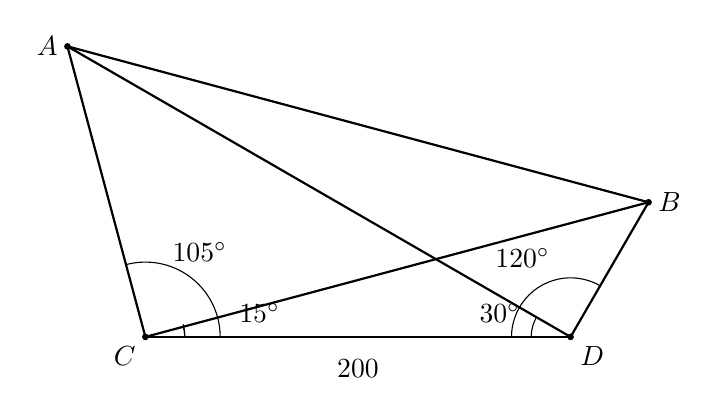
\begin{tikzpicture}[scale=1.0]
  \coordinate (C) at (0,0);
  \coordinate (D) at (5.4,0);
  \coordinate (A) at (-0.99,3.69);
  \coordinate (B) at (6.39,1.71);
  \draw[thick] (A)--(B);
  \draw[thick] (A)--(C);
  \draw[thick] (A)--(D);
  \draw[thick] (B)--(C);
  \draw[thick] (B)--(D);
  \draw[thick] (C)--(D);
  \draw (0.95,0) arc[start angle=0,end angle=105,radius=0.95];
  \draw (0.5,0) arc[start angle=0,end angle=15,radius=0.5];
  \draw (0.5,0) arc[start angle=0,end angle=15,radius=0.62];
  \draw ([shift=(180:0.5)]D) arc[start angle=180,end angle=150,radius=0.5];
  \draw ([shift=(180:0.75)]D) arc[start angle=180,end angle=60,radius=0.75];
  \fill (A) circle (1.2pt) node[left] {$A$};
  \fill (B) circle (1.2pt) node[right] {$B$};
  \fill (C) circle (1.2pt) node[below left] {$C$};
  \fill (D) circle (1.2pt) node[below right] {$D$};
  \node at (0.69,1.08) {$105^\circ$};
  \node at (1.45,0.30) {$15^\circ$};
  \node at (4.5,0.30) {$30^\circ$};
  \node at (4.79,1.00) {$120^\circ$};
  \node at (2.7,-0.4) {$200$};
\end{tikzpicture}
\end{center}
\nopagebreak[4]
\end{question}
\begin{question}
\gkti{6}已知直线 $4x+3y-12=0$ 和园心在 $(4,7)$ 点的一个园相切，求这园的半径及过园心和切点的直线方程。

\textbf{参考题 1．} 把 $4x^2+9y^2+8x-36y+4=0$ 化成标准方程，并指出它所代表的曲线的长、短半轴、离心率。

\textbf{参考题 2．} 试求下列各式的导数：

（1）$y=3x^2+\sqrt{x}+5$；

（2）$y=\ln(x^{10})+\ln(\ln x)$；

（3）$y=x^x$。

\textbf{参考题 3．} 求微分方程的通解：

（1）$y'=\dfrac{2+y}{3-x}$；

（2）$y''-2y'-3y=0$。

\end{question}